% =========================
% File: main.tex (FINAL)
% =========================

\documentclass[11pt,a4paper]{article}

% ---------- Packages ----------
\usepackage[margin=1in]{geometry}
\usepackage{amsmath,amssymb}
\usepackage{graphicx}
\usepackage{subcaption}
\usepackage{booktabs}
\usepackage{hyperref}
\usepackage{siunitx}
\usepackage{enumitem}
\usepackage{microtype}
\usepackage{float}
\usepackage{caption}

\hypersetup{
    colorlinks=true,
    linkcolor=blue,
    citecolor=blue,
    urlcolor=blue
}

\setlength{\parindent}{0pt}
\setlength{\parskip}{0.6em}

% ---------- Title ----------
\title{\textbf{Synapse — Analytical Report: Signals, Models, and Methods}\\
\large Robust Subject-Independent 8-Channel sEMG Gesture Recognition}

\author{Keerthi Kumar K J}
\date{} % intentionally empty (competition-clean)

\begin{document}
\maketitle

% ---------- Abstract ----------
\begin{abstract}
This report presents a subject-independent framework for classifying gestures from 8-channel surface electromyography (sEMG) signals. We focus on interpreting the received biosignals, motivating each signal processing step based on observed signal properties, and justifying the selected machine learning architectures through physiological and statistical reasoning. A leakage-safe preprocessing pipeline, robust normalization, and a soft-voting ensemble of complementary neural models are employed. Emphasis is placed on the rationale behind every methodological choice and on the inferences drawn from both processed signals and model outputs, in alignment with real-world deployment constraints.
\end{abstract}

\tableofcontents
\clearpage

% =========================================================
\section{Signal Interpretation and Physiological Meaning}
% =========================================================

\subsection{Nature of surface EMG signals}
Surface electromyography measures the superimposed electrical activity generated by motor unit action potentials during muscle contraction. Unlike stationary biomedical signals, sEMG exhibits strong temporal non-stationarity, burst-like activation patterns, and subject-dependent amplitude characteristics.

From exploratory inspection of the dataset, several defining properties emerge:
\begin{itemize}[noitemsep]
    \item \textbf{Non-stationary temporal structure}: distinct onset, sustain, and offset phases for each gesture.
    \item \textbf{Broadband frequency content}: dominant energy concentrated approximately between \SI{20}{Hz} and \SI{450}{Hz}.
    \item \textbf{Heavy-tailed amplitude distributions}: caused by motion artifacts, electrode shifts, and transient spikes.
    \item \textbf{High inter-subject variability}: absolute signal amplitude and activation timing differ substantially across users.
\end{itemize}

These characteristics motivate robust preprocessing and temporal modeling strategies rather than reliance on absolute amplitude cues, which are known to generalize poorly across subjects \cite{emg_survey}.

\subsection{Exploratory signal evidence}
Figure~\ref{fig:raw_psd} visualizes a raw multi-channel sEMG segment alongside its power spectral density, while Figure~\ref{fig:spec} illustrates time–frequency localization of muscle activity. The observed burst dynamics and spectral concentration directly inform subsequent filtering, normalization, and model design choices.

\begin{figure}[H]
  \centering
  \begin{subfigure}[t]{0.48\textwidth}
    \includegraphics[width=\textwidth]{figures/fig_raw_snippet.png}
    \caption{Raw 8-channel sEMG snippet (stacked).}
    \label{fig:raw}
  \end{subfigure}
  \hfill
  \begin{subfigure}[t]{0.48\textwidth}
    \includegraphics[width=\textwidth]{figures/fig_psd.png}
    \caption{Welch power spectral density per channel.}
    \label{fig:psd}
  \end{subfigure}
  \caption{Exploratory analysis revealing non-stationarity and broadband spectral content.}
  \label{fig:raw_psd}
\end{figure}

\begin{figure}[H]
  \centering
  \includegraphics[width=0.85\textwidth]{figures/fig_spectrogram.png}
  \caption{Representative STFT spectrogram showing temporally localized muscle activation bursts.}
  \label{fig:spec}
\end{figure}

% =========================================================
\section{Signal Processing Methods and Rationale}
% =========================================================

The signal processing pipeline is explicitly designed to suppress nuisance variability while preserving gesture-discriminative temporal morphology.

\subsection{Filtering and detrending}
A zero-phase bandpass filter in the range \SIrange{20}{450}{Hz} is applied to remove baseline drift and high-frequency noise. When powerline interference is detected in the PSD, a narrow notch filter at 50/60 Hz is applied.

\textbf{Rationale:} The selected passband preserves the physiological frequency range of motor unit activity while eliminating components unrelated to muscle contraction, as evidenced by Fig.~\ref{fig:psd}.

\subsection{Windowing strategy}
Signals are segmented into fixed windows of length $L=256$ samples with stride $S=128$ (50\% overlap).

\textbf{Rationale:} A 256-sample window captures the complete temporal evolution of a typical gesture (activation onset to release), while overlap increases sample density and improves temporal continuity at decision boundaries.

\subsection{Robust normalization using Median--IQR scaling}
For each channel, normalization is performed using statistics computed exclusively on the training folds:
\[
\tilde{x} = \frac{x - \mathrm{median}(x)}{\max(\mathrm{IQR}(x), \epsilon)}
\]
where $\mathrm{IQR}(x) = Q_3 - Q_1$.

\textbf{Rationale:} Unlike mean–variance normalization, Median--IQR scaling is resistant to extreme artifacts and heavy-tailed distributions \cite{robust_stats}. This forces models to rely on temporal structure rather than spurious amplitude outliers, improving subject-independent generalization.

\subsection{Data augmentation}
Training-only augmentations include small additive noise, channel dropout, mild temporal jitter, and per-channel gain scaling.

\textbf{Inference:} These augmentations simulate realistic acquisition variability (electrode shift, sensor noise) and reduce overfitting to subject-specific signal statistics.

% =========================================================
\section{Machine Learning Approach and Model Architecture}
% =========================================================

\subsection{Validation protocol}
We employ 5-fold GroupKFold cross-validation, grouping samples by subject identity.

\textbf{Rationale:} Random splits leak subject-specific information and yield over-optimistic results. Group-wise validation ensures that reported performance reflects true generalization to unseen users.

\subsection{Model architectures and design rationale}
Three complementary architectures are trained and combined via soft voting (Fig.~\ref{fig:arch}).

\subsubsection{NeuroCNN}
A compact 1D convolutional network extracts local temporal patterns and inter-channel correlations.

\textbf{Rationale:} CNN filters efficiently detect short-lived transients and spatial co-activation patterns across electrodes.

\subsubsection{NeuroResNet}
A deeper residual network learns hierarchical abstractions while maintaining stable optimization.

\textbf{Rationale:} Residual connections mitigate gradient degradation, enabling the network to model more complex signal morphologies \cite{resnet}.

\subsubsection{NeuroTCN}
A Temporal Convolutional Network with exponentially increasing dilations ($d=1,2,4,\dots,64$) and kernel size $k=3$.

The receptive field is:
\[
\mathrm{RF} = 1 + (k-1)\sum_{i=0}^{6} 2^i = 255
\]

\textbf{Inference:} The receptive field matches the window length (256), allowing the model to condition each prediction on the entire gesture history, a critical requirement for non-stationary sEMG signals \cite{tcn}.

\subsection{Soft-voting ensemble}
Predicted class probabilities from all 15 trained models (3 architectures × 5 folds) are averaged.

\textbf{Rationale:} Ensembling reduces variance and mitigates architecture-specific failure modes, yielding more stable predictions under subject and session variability.

\begin{figure}[H]
  \centering
  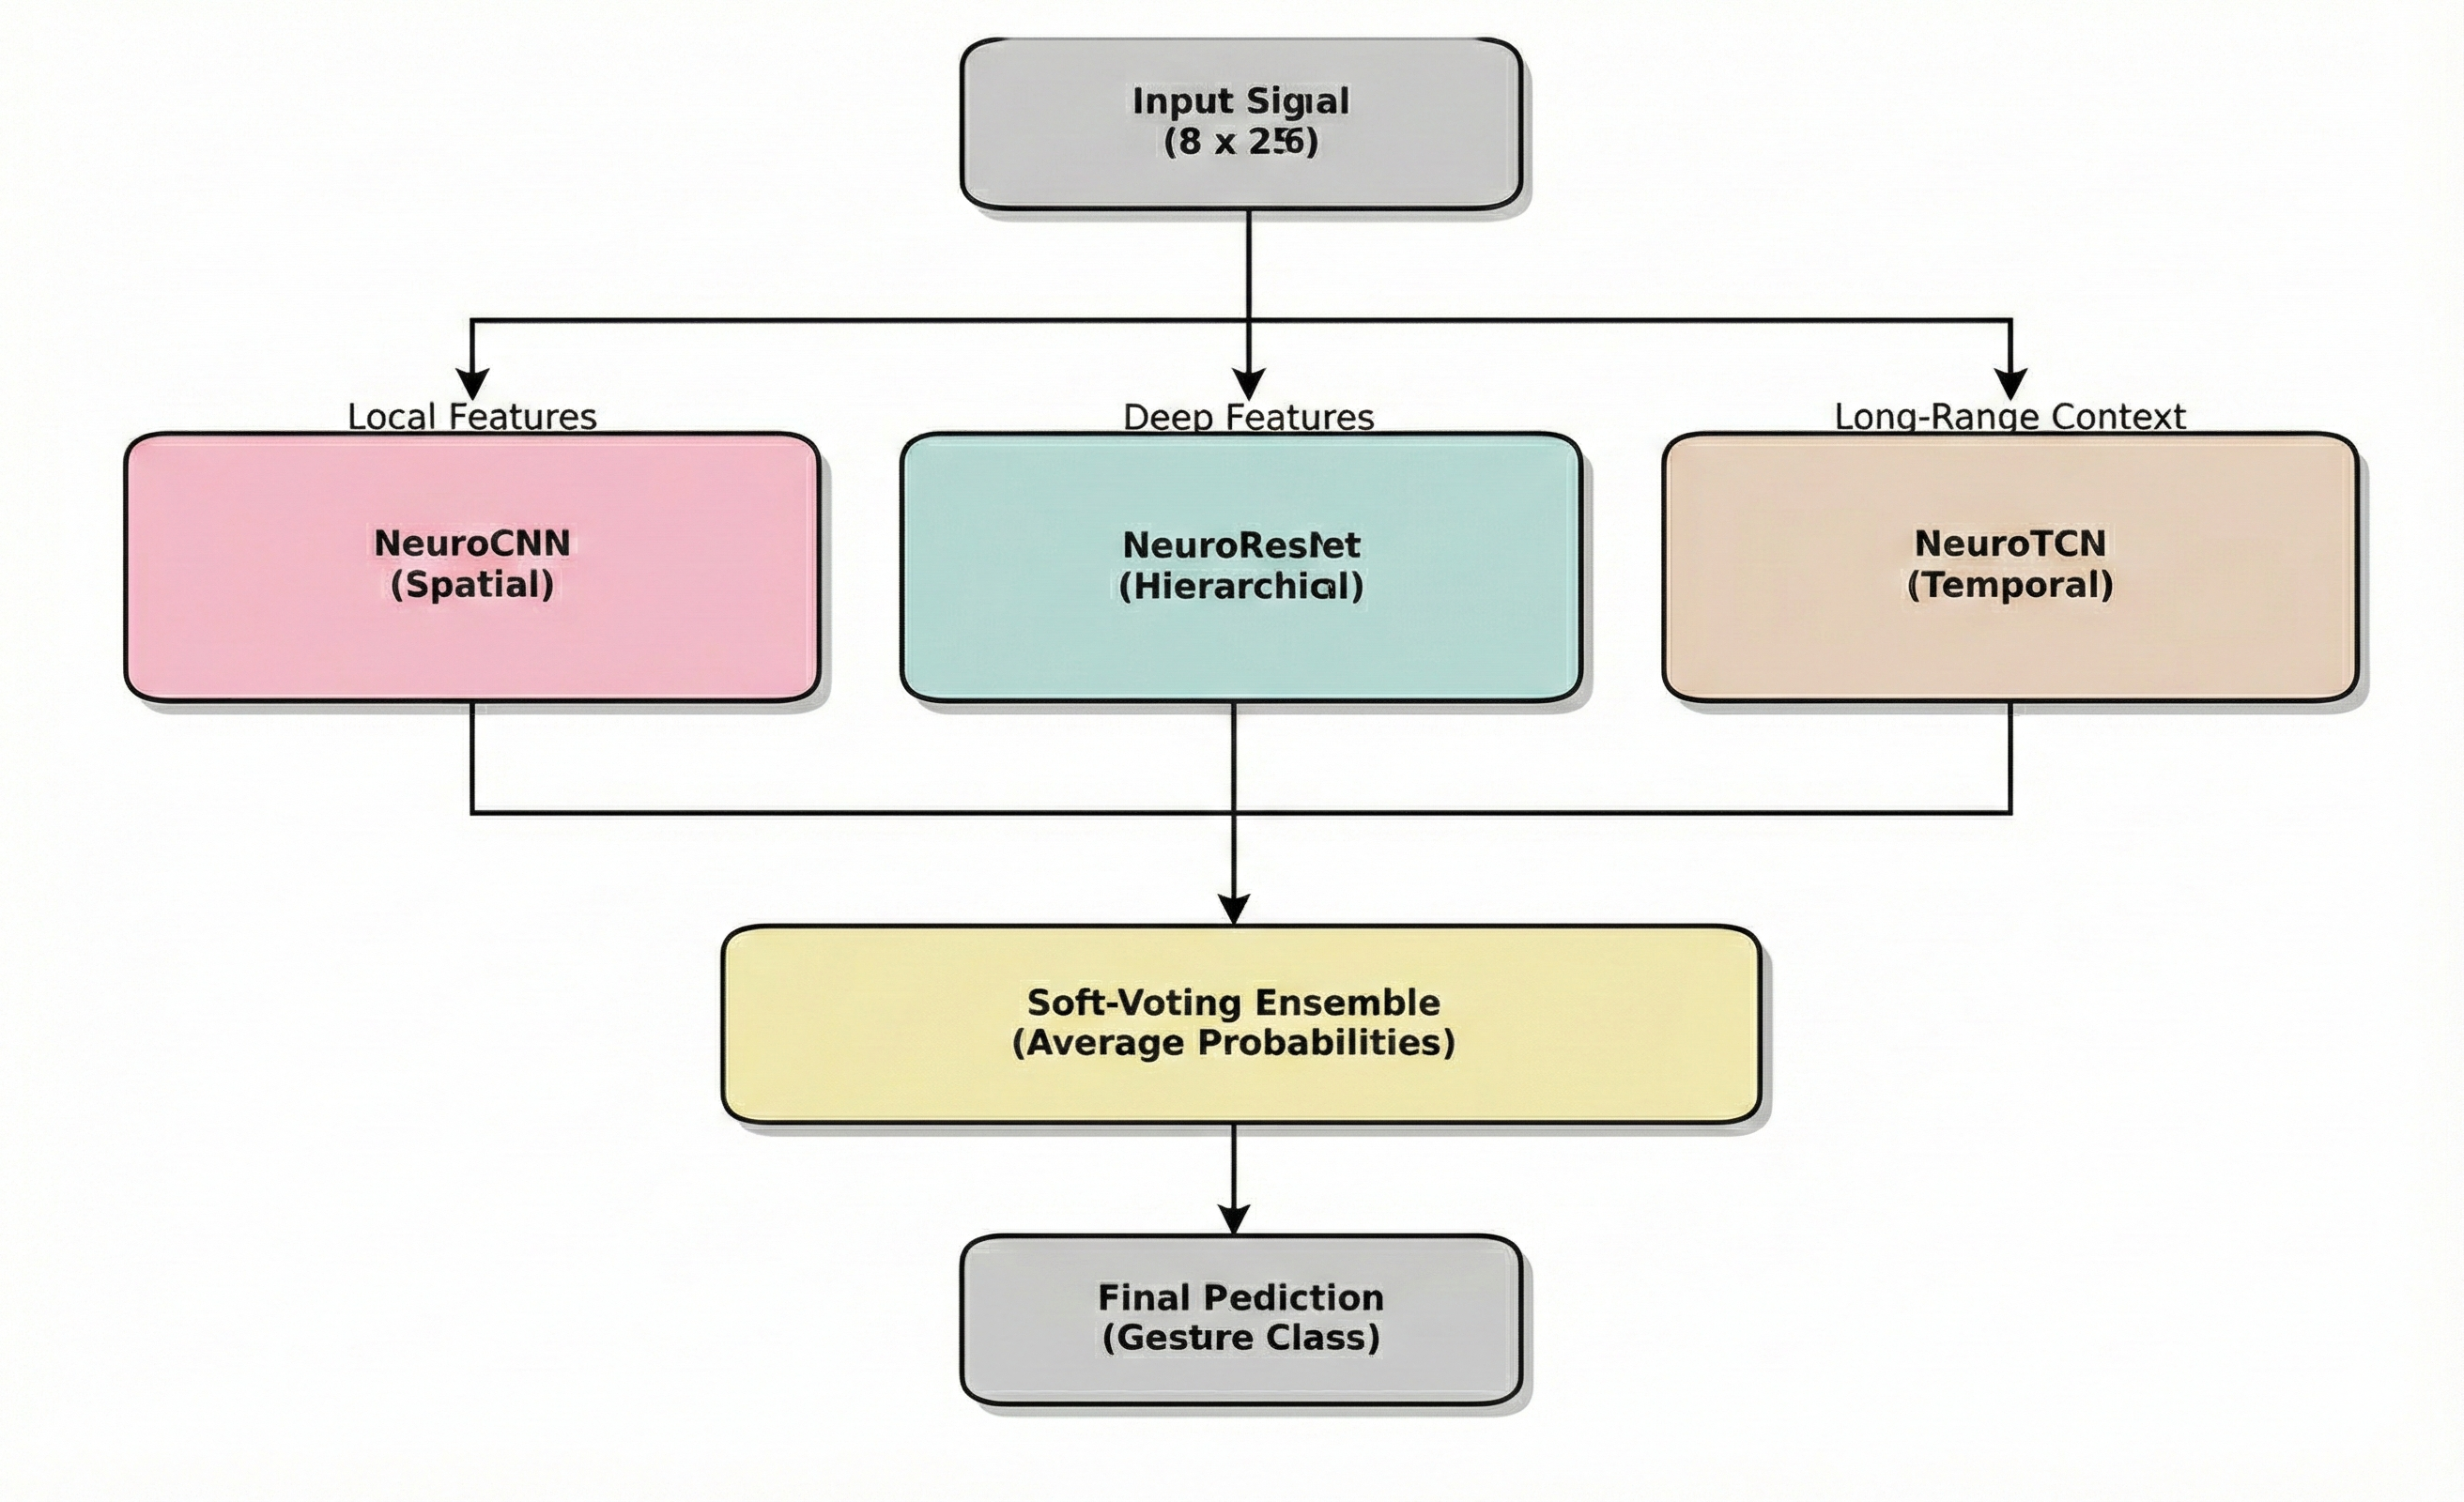
\includegraphics[width=0.85\textwidth]{figures/fig_architecture.png}
  \caption{Soft-voting ensemble of NeuroCNN, NeuroResNet, and NeuroTCN architectures.}
  \label{fig:arch}
\end{figure}

% =========================================================
\section{Results and Inferences from Processed Signals}
% =========================================================

\subsection{Cross-subject stability}
Figure~\ref{fig:results} (left) shows consistent F1 scores across folds with low variance, indicating effective normalization and subject-independent learning.

\subsection{Error analysis}
The normalized confusion matrix (Fig.~\ref{fig:results}, right) exhibits strong diagonal dominance. Residual confusions occur between biomechanically similar gestures, whose spectro-temporal signatures partially overlap (cf. Fig.~\ref{fig:spec}).

\textbf{Inference:} Errors correlate with genuine physiological similarity rather than modeling artifacts, suggesting that further gains would require higher spatial resolution or adaptive personalization rather than architectural changes.

\begin{figure}[H]
  \centering
  \begin{subfigure}[t]{0.48\textwidth}
    \includegraphics[width=\textwidth]{figures/fig_training_curves.png}
    \caption{Fold-wise F1 stability.}
  \end{subfigure}
  \hfill
  \begin{subfigure}[t]{0.48\textwidth}
    \includegraphics[width=\textwidth]{figures/fig_confusion_matrix.png}
    \caption{Normalized confusion matrix.}
  \end{subfigure}
  \caption{Quantitative evaluation and inference.}
  \label{fig:results}
\end{figure}

% =========================================================
\section{Conclusion}
% =========================================================

By explicitly linking physiological signal properties to preprocessing decisions, normalization strategy, temporal receptive field design, and validation protocol, this work prioritizes robustness over fragile peak accuracy. The proposed ensemble demonstrates stable subject-independent performance and offers a practical foundation for real-world neurotechnology deployment.

% =========================================================
\appendix
\section{Reproducibility Summary}
The submission includes the \texttt{main.tex} source, compiled PDF, trained model checkpoints with corresponding scalers, preprocessing and inference scripts, and all figures required to reproduce the reported results.

% =========================================================
\begin{thebibliography}{9}

\bibitem{tcn}
S.~Bai, J.~Z. Kolter, and V.~Koltun,
``An empirical evaluation of generic convolutional and recurrent networks for sequence modeling,''
\textit{arXiv:1803.01271}, 2018.

\bibitem{resnet}
K.~He, X.~Zhang, S.~Ren, and J.~Sun,
``Deep residual learning for image recognition,''
\textit{Proc. CVPR}, 2016.

\bibitem{emg_survey}
A.~Phinyomark, P.~Phukpattaranont, and C.~Limsakul,
``Feature reduction and selection for EMG signal classification,''
\textit{Expert Systems with Applications}, 2012.

\bibitem{robust_stats}
P.~J. Huber,
\textit{Robust Statistics},
John Wiley \& Sons, 1981.

\end{thebibliography}

\end{document}
